\begin{figure}[t]
\centering
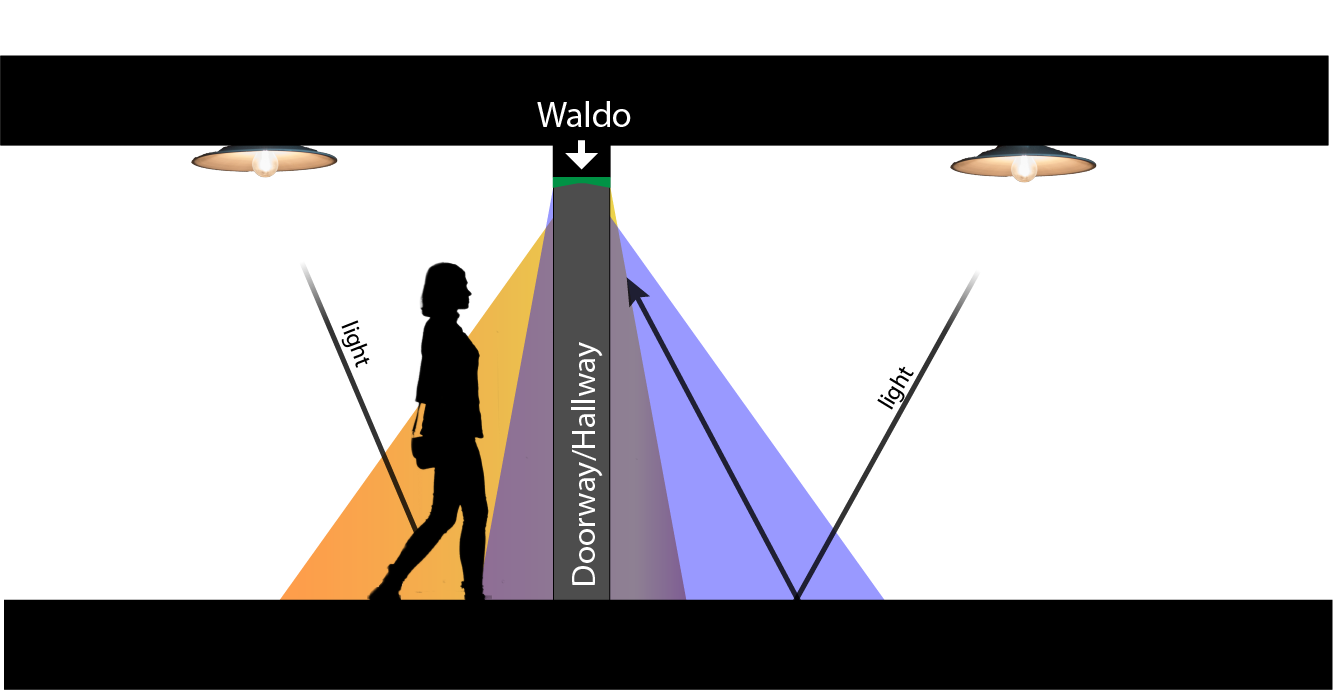
\includegraphics[width=0.9\columnwidth]{figs/scenario2.png}
\caption{ The overall system concept of \sysname, a batteryless, energy-harvesting, doorway mounted occupancy tracking and person detection enabling system.  This system uses reflective indoor lighting to both power the system and detect person entry and exit activity to a room or corridor.\label{fig:syspic}}
\end{figure}

\section{Introduction}
\label{sec:intro}

% intro to occupancy tracking
Understanding how people move, work, and live within a workplace or residence is essential for enabling health, efficiency, and security applications in smart buildings.
Appliances, computers, lighting, heating and cooling systems can adapt their behavior depending on the number of occupants, their needs, and the context of their interactions.
Smart buildings can automatically identify indoor traffic patterns, poorly-used space, and congested walkways, helping us better understand how people interact with the indoor spaces they use.
We can only achieve these benefits if we can effectively sense how people move indoors.


%\fxnote{[I had hard time  reading from this point to "our solution" first you gave the reader some disadvantages of existing systems. Then you jumped to give an examples about different approaches for these systems , Then you continue in giving the disadvantages - I suggest to give examples of existing systems and then list their issues-AA]}
Unfortunately, current occupancy-tracking systems are large, expensive, and high-maintenance---too expensive for large-scale deployments and too high-maintenance for long-term use.
%
Existing systems use a variety of techniques, including ultrasound\cite{hnat2012doorjamb}, images\cite{tyndall2016occupancy, teixeira2007lightweight}, wearables\cite{fishkin2005hands}, instrumented objects\cite{buettner2009activity}, structural vibrations\cite{pan2016occupant}, and opportunistic data leaked from existing meters and security systems\cite{yangoccupancy2014}.
Some gather identifiable information.  %\fxnote{[Might need to mention the networking paper's work or maybe it being in the related work is sufficient -NT]}
Others require building remodeling, force users to change their behavior, or require structural models of the building.
For any of these solutions to work, we must either provide wired power to the sensors (which is usually both expensive and invasive), or use batteries which increase cost, environmental impact, and fire risk, and which must be replaced every few years~(even rechargeables).

% our solution
In this paper we present \sysname (overview shown in \figref{fig:syspic}), an occupancy-monitoring sensor that is low-cost and low-maintenance, preserves occupant privacy, and can operate for decades\footnote{Actual lifetimes depend on environmental conditions, enclosure quality, and rates of decay for silicon and other circuit materials. Without the usual bottleneck (the battery), lifetimes of 10--50 years are realistic but not guaranteed.} without wired power or batteries.
%

% why batteryless?
%Importantly, \sysname is batteryless to enable the long term deployment at scales required to instrument entire commercial buildings and residential neighborhoods.
%Batteries are expensive, bulky, environmentally unsustainable, and do not have long lifetimes (even rechargeables).
%By leaving the batteries behind, the device power supply becomes intermittent, complicating execution, data collection, energy management, and timekeeping.
%However, the ability for long term deployments at the scales envisioned for the Internet-of-Things provides enough motivation.

Like previous solutions~\cite{hnat2012doorjamb}, \sysname attaches to the top of a door frame and monitors movement in and out of the doorway.
In contrast, however, \sysname does not use active sensors~(like ultrasonic range finders), but instead senses movement using the same ambient light reflections that power the sensor.
\sysname harvests solar energy from indoor lights to power all operations, and uses a combination of hardware and software techniques to detect human movement and direction as solar energy availability changes.
%Besides harvesting solar energy, \sysname processes in hardware and software the signal generated by an array of solar panels to detect when people enter or exit a room.
%When enough energy is available, and a person is walking through the doorway, \sysname uses ultrasonic range finders to measure the height of the person for identification.
\sysname stores this information on device, and opportunistically transmits occupancy information to a basestation using its radio.


%Because of the incredibly tight energy constraints and unpredictable energy-harvesting conditions, \sysname uses approximate computing concepts to provide value to the global system no matter the energy conditions.
%\sysname dynamically adapts its duty cycle, task schedule, and data-transmission granularity, depending on the energy available.
%If relatively high amounts of energy are available in the environment, then \sysname will use the ranging sensor to get heights for each person passing through the doorway, and will send each passing event over the air through BLE to the basestation.
%If relatively low amounts of energy are available in the environment, then \sysname will turn off the range finder, and use only the passive, zero-energy-cost solar panels to detect passing events.
%Instead of transmitting on each passing event in this low energy state, \sysname instead sends global statistics opportunistically, detailing the number of events or people that have passed since the last interaction.


%\subsection*{Contributions}
\noindpar{Contributions:}

%\begin{compactenum}
\begin{enumerate}[label=\arabic*., align=left, leftmargin=*]
	\item We present a novel system design for unobtrusive, long-term, low-cost, zero-maintenance occupancy tracking.
	\item We explore design considerations for batteryless, intermittently-powered sensing systems for detecting ephemeral events that can be broadly applied to other batteryless sensing applications.
	%\item A novel approximate computing method for adapting the duty cycle of batteryless occupancy  sensors depending on energy available, trading off accuracy for energy.
%\fxnote{[We need to reword this - HD]} %  1) record heights, 2) then record each event and report, 3) only report stats of people going in and out
	%\item An investigation of security and privacy considerations stemming from ubiquitous, low cost occupancy sensors.
	\item We provide an implementation, deployment (both controlled and in-the-wild), and evaluation of \sysname that explores the strengths and limitations of our approach. 
%\end{compactenum}
\end{enumerate}

\noind
\sysname is, to our knowledge, the first batteryless occupancy-monitoring solution~\cite{desai2018, sorber_tobias_2022}, and demonstrates the potential and usefulness of long-lived, energy-harvesting, batteryless sensing operation in the built environment. %\fxnote{[I'm waffling between simply saying as we had that we were the first and citing the patent... which is here but also could simply say "the first single sensor batteryless occupancy-monitoring system solution" - could be worded better or maybe I'm just overthinking this.  Let me know what you all think here.  -NT]}
In this paper we present our design, a working prototype, and evaluation results showing the efficacy of the approach.


% These types of condensed table of contents in papers communicate essentially nothing, let's not waste the space - JDH
%\noind
%In the following sections, we give background and related works on occupancy detection and batteryless sensing (\secref{sec:background}), outline the \sysname system design (\secref{sec:system}) and implementation (\secref{sec:implementation}), demonstrate the feasibility and general applicability of \sysname in a variety of situations (\secref{sec:evaluation}), discuss limitations, privacy considerations, and future work (\secref{sec:discussion}), and conclude (\secref{sec:conclusions}).
